\section{Future Work}

\subsection{Generated Data}
\begin{frame}{Simulating \textit{"real data"}}
We have taken several precautions when generating data:
\begin{itemize}
\item Randomizing destinations
\item Pertubation of GPS data
\item Randomized GPS-update-time
\end{itemize}
Introduced to enforce the development of a system capable of dealing with data-variation\\
Randomization is based on even probability distribution
\begin{itemize}
\item Convergence of generated data
\end{itemize}
\end{frame}

\begin{frame}{Route convergence}
\begin{center}
\fbox{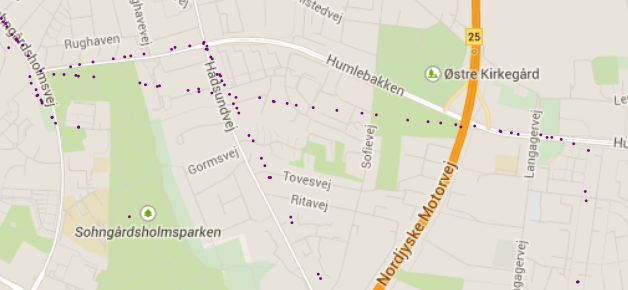
\includegraphics[width=0.7\textwidth]{graphics/convergence}}
\end{center}
\begin{itemize}
\item No \textit{''off-route''} cycling
\item Routes are defined by points
\end{itemize}
\end{frame}

\begin{frame}{Hotspot convergence}
\begin{center}
\fbox{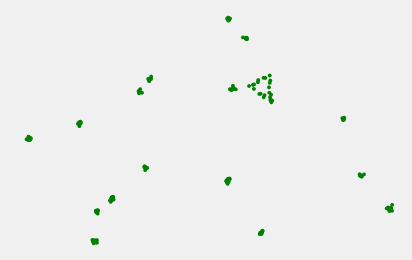
\includegraphics[height=10em]{graphics/convergence2}}
\fbox{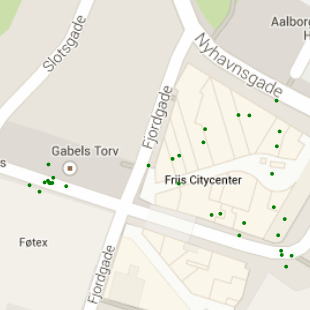
\includegraphics[height=10em]{graphics/convergence3}}
\end{center}
\begin{itemize}
\item All routes end at pre-determined locations
\item No bikes left at random places
\end{itemize}
\end{frame}
%randomized destinations
%random yet clean (data converges to neat hotspots. no off-path cycling. no bikes left at random places)

\subsection{Aalborg Kommune}
\begin{frame}{Requested information}
Queries proposed by Aalborg Kommune:
\begin{itemize}
\item What routes are travelled?
\item How long are the trips?
\item When are bikes used?
\item Who uses the bikes?
\end{itemize}\vspace{1em}
None are supported by current API
\begin{itemize}
\item Current API is end-user only
\end{itemize}
\end{frame}

%\subsection{Usage Statistics}
%\subsection{API Access Levels}
\subsection{Spatial Querying}
\begin{frame}{Data structure}{}
{
\setbeamercolor{block title}{use=structure,fg=white,bg=purple!75!black}
\begin{block}{Problem:}
Determining hotspot for a GPS point is inefficient.
\end{block}
}
\begin{block}{Solution 1:}
Apply a different clustering algorithm that performs hierarchical clustering.
\end{block}
\begin{block}{Solution 2:}
Organize hotspots in a structure optimized for spatial queries such as an R-Tree.
\end{block}
\end{frame}

\subsection{Multiple Models}
\begin{frame}{Incomplete}
When to create new models?
\end{frame}